\documentclass[11pt,a4paper]{article}

\usepackage[margin=1in]{geometry}
\usepackage[T1]{fontenc}
\usepackage[utf8]{inputenc}
\usepackage{lmodern}
\usepackage{microtype}
\usepackage{hyperref}
\usepackage{xcolor}
\usepackage{booktabs}
\usepackage{longtable}
\usepackage{array}
\usepackage{enumitem}
\usepackage{listings}
\usepackage{tcolorbox}
\usepackage{tabularx}
\usepackage{tikz}
\usepackage{fancyhdr}
\usepackage{lastpage}
\usepackage{titlesec}
\usepackage{caption}
\usepackage{float}
\usetikzlibrary{arrows.meta,positioning,fit,shapes.geometric,calc}

\hypersetup{
  colorlinks=true,
  linkcolor=blue!60!black,
  urlcolor=blue!60!black,
  citecolor=blue!60!black,
  pdftitle={Agentic AI Exam Grader Technical Design Document},
  pdfauthor={Erfan Babakhani}
}

\definecolor{darkblue}{HTML}{17365D}
\definecolor{lightblue}{HTML}{EAF2F8}
\definecolor{lightgray}{HTML}{F5F5F5}
\definecolor{darkgreen}{HTML}{1B5E20}
\definecolor{warn}{HTML}{FFF4E5}
\definecolor{danger}{HTML}{FDEDEC}

\titleformat{\section}{\Large\bfseries\color{darkblue}}{\thesection}{0.75em}{}
\titleformat{\subsection}{\large\bfseries\color{darkblue}}{\thesubsection}{0.75em}{}
\titleformat{\subsubsection}{\normalsize\bfseries\color{darkblue}}{\thesubsubsection}{0.75em}{}

\pagestyle{fancy}
\fancyhf{}
\lhead{Agentic AI Exam Grader}
\rhead{Technical Design}
\cfoot{Page \thepage}

\lstdefinestyle{code}{
  basicstyle=\ttfamily\small,
  backgroundcolor=\color{lightgray},
  frame=single,
  breaklines=true,
  columns=fullflexible,
  showstringspaces=false,
  keepspaces=true,
  tabsize=2,
  rulecolor=\color{gray!60}
}
\lstset{style=code}

\setlength{\headheight}{14pt}
\lstdefinelanguage{json}{
  basicstyle=\ttfamily\small,
  showstringspaces=false,
  breaklines=true,
  literate=
   *{0}{{{0}}}{1}{1}{{{1}}}{1}{2}{{{2}}}{1}{3}{{{3}}}{1}{4}{{{4}}}{1}
    {5}{{{5}}}{1}{6}{{{6}}}{1}{7}{{{7}}}{1}{8}{{{8}}}{1}{9}{{{9}}}{1}
    {:}{{{\color{black}:}}}{1}{,}{{{\color{black},}}}{1}
    {\{}{{{\{}}}{1}{\}}{{{\}}}}{1}{[}{{{[}}}{1}{]}{{{]}}}{1},
}


\newtcolorbox{decisionbox}{colback=lightblue,colframe=darkblue,title=Design Decision,arc=2mm,boxrule=0.7pt}
\newtcolorbox{riskbox}{colback=danger,colframe=red!60!black,title=Rejection / Risk Note,arc=2mm,boxrule=0.7pt}
\newtcolorbox{notebox}{colback=warn,colframe=orange!80!black,title=Implementation Note,arc=2mm,boxrule=0.7pt}

\newcommand{\code}[1]{\texttt{\detokenize{#1}}}

\begin{document}

\begin{titlepage}
  \centering
  \vspace*{1.2cm}
  {\Huge\bfseries Agentic AI Exam Grader\\[0.35em]Technical Design Document\par}
  \vspace{0.5cm}
  {\Large Backend-only take-home implementation plan\par}
  \vspace{1.2cm}
  \begin{tcolorbox}[colback=lightblue,colframe=darkblue,width=0.86\textwidth,arc=2mm]
  \textbf{Purpose.} This document specifies a complete backend-only implementation for a minimal AI exam grader. The system accepts an exam PDF containing questions plus official marking material and a handwritten student-answer PDF, then returns a structured per-question grading result using the provisioned Azure OpenAI deployment configured for \code{gpt-5.4-mini}. It is designed to satisfy the assignment's non-negotiable rejection rules while preserving a controlled agentic grading pipeline.
  \end{tcolorbox}
  \vfill
  \begin{tabular}{rl}
    \textbf{Author:} & Armin Khosravi \\
    \textbf{Scope:} & Backend, API, database, Docker, agentic grading pipeline \\
    \textbf{Frontend:} & Intentionally out of scope for the first submission \\
    \textbf{Primary model:} & Azure OpenAI deployment \code{gpt-5.4-mini} only \\
    \textbf{Status:} & Implementation-ready design \\
  \end{tabular}
  \vfill
  {\small This document is intended to be placed in the project repository as an architecture/design reference in addition to the root \code{README.md}.}
\end{titlepage}

\tableofcontents
\newpage

\section{Executive Summary}

The proposed system is a \textbf{controlled agentic grading workflow} implemented behind a conventional backend API. It is not a single prompt that blindly sends two PDFs to a model. It is also not an unconstrained autonomous multi-agent system. Instead, it uses a fixed, inspectable workflow for reliability, and bounded agentic behavior only where dynamic tool use is genuinely useful: locating handwritten answers, cropping and zooming difficult regions, and interpreting non-standard student solutions.

The backend exposes authentication and grading endpoints, persists all grading runs per user, enforces a hard 120-second request limit, and uses only the provisioned Azure OpenAI deployment. The grading workflow parses the exam and official solution, infers a transparent rubric when explicit marks are absent, inspects handwritten student work using vision-first PDF processing, grades each answer against rubric criteria, validates novel but correct solution paths, repairs inconsistent structured outputs, and stores a complete result with evidence references.

\begin{decisionbox}
The core design principle is: \textbf{workflow for reliability, bounded agents for perception and ambiguity}. The overall route is deterministic, while the student-answer inspection step is allowed to use ReAct-style tool selection over a small set of local tools such as page rendering, cropping, and zooming.
\end{decisionbox}

\section{Required Source Documents Before Implementation}

Before coding, the implementer must read two assignment documents in full:

\begin{enumerate}[leftmargin=*]
  \item \textbf{\code{INTERN_TAKEHOME.pdf}}: defines the product requirements, required endpoints, rejection rules, output expectations, and optional bonuses.
  \item \textbf{\code{API_QUICKSTART.pdf}}: defines the Azure OpenAI environment variables, endpoint, API version, exact deployment name, and the requirement to use the Azure OpenAI client instead of the public OpenAI client.
\end{enumerate}

The API quickstart should be treated as an implementation constraint, not a general example. The application should load these values from environment variables:

\begin{lstlisting}
AZURE_OPENAI_API_KEY=<provided separately>
AZURE_OPENAI_ENDPOINT=https://zanistagpteastus2.openai.azure.com/
AZURE_OPENAI_DEPLOYMENT=gpt-5.4-mini
AZURE_OPENAI_API_VERSION=2024-12-01-preview
\end{lstlisting}

The quickstart states that \code{gpt-5.4-mini} is multimodal and accepts text and images. This supports the design decision to render handwritten student PDFs to page images and send relevant images or crops to the Azure deployment. The quickstart also states that calling any other deployment is an automatic rejection. Therefore, all model access must go through a single Azure client wrapper with no fallback model and no per-call deployment override.

\begin{riskbox}
Do not start implementation from memory alone. Re-read \code{API_QUICKSTART.pdf} before wiring the Azure client, because the endpoint, API version, deployment name, and request format are assignment-specific.
\end{riskbox}

\section{Assignment Requirements Interpreted as Engineering Constraints}

The assignment requires a minimal AI exam grader. The inputs are an exam paper PDF containing questions plus the official mark scheme and a handwritten student-answer PDF. The output must be a structured grading result produced with the provisioned \code{gpt-5.4-mini} deployment. At minimum, every grading run must include awarded and maximum marks per question, a total score, and per-question feedback. The output must be machine-readable and complete: every question in the exam must appear in the output, including blank or unanswered questions.

The non-negotiable rejection rules are treated as hard engineering constraints rather than nice-to-have items. The design therefore includes explicit support for Docker Compose, backend HTTP APIs, authentication, password hashing, persistent per-user database storage, hard cancellation at 120 seconds, Azure environment variables, model restriction, and root-level documentation.

\subsection{Non-negotiable Requirement Mapping}

\begin{longtable}{p{0.28\textwidth}p{0.65\textwidth}}
\toprule
\textbf{Requirement} & \textbf{Design Response} \\
\midrule
Runs from a clean clone with \code{docker compose up} & A root \code{docker-compose.yml} builds the backend image, starts the API service, and mounts a persistent volume for SQLite or connects to Postgres. No manual dependency installation is required. \\
Backend HTTP API & Django REST Framework exposes all required endpoints under \code{/api}. The frontend is implemented separately in Next.js and documented in the root README. \\
Register / login / submit grading / list past gradings / retrieve grading & Implemented as \code{POST /auth/register}, \code{POST /auth/login}, \code{POST /gradings}, \code{GET /gradings}, and \code{GET /gradings/\{id\}}. \\
Real authentication & Protected routes require a valid server-issued bearer token. Authorization is checked server-side against database ownership. \\
Passwords hashed & Passwords are stored only as strong hashes using Argon2 or bcrypt. Raw passwords are never persisted or logged. \\
Persistence in database & Grading runs, uploaded file metadata, parsed questions, rubrics, grades, evidence, and overrides are persisted in a database that survives container restarts. \\
Per-user scoping & Every grading run is linked to \code{user_id}; list/retrieve queries filter by the authenticated user. Cross-user access returns 404 or 403. \\
Hard request limit: 120 seconds & The orchestrator is wrapped in a real cancellation boundary. If the budget expires, local tools and pending LLM calls are cancelled where possible and the endpoint returns HTTP 504. \\
Use only \code{gpt-5.4-mini} deployment & The Azure client reads a single deployment name from \code{AZURE_OPENAI_DEPLOYMENT}; no fallback model, embedding model, OCR cloud model, or alternate deployment is called. \\
Credentials from environment variables & API key, endpoint URL, deployment name, and API version are read from env vars. No secrets are committed or baked into the Docker image. \\
No secrets, \code{.env}, or DB files committed & \code{.gitignore} excludes \code{.env}, SQLite files, uploads, rendered pages, caches, and logs. Only \code{.env.example} is committed. \\
Root README & The README documents setup, env vars, endpoints, database behavior, design choices, known limitations, AI-tool usage, and testing. \\
\bottomrule
\end{longtable}

\section{Observed Properties of the Sample Data}

The uploaded sample bundle contains one exam/solution PDF and seven student-answer PDFs. The important observation is that the student-answer PDFs are not reliably machine-readable as text. Several contain zero extractable text. Others contain partial text, usually only the typed exam prompt, while the handwritten answer remains unavailable to text extraction. This strongly motivates a vision-first or hybrid text-image design.

\begin{longtable}{p{0.36\textwidth}p{0.13\textwidth}p{0.15\textwidth}p{0.28\textwidth}}
\toprule
\textbf{File} & \textbf{Pages} & \textbf{Text extraction} & \textbf{Implication} \\
\midrule
\code{Homework_3_sols.pdf} & 2 & Extractable & Use text plus rendered pages to parse questions and official solutions. \\
\code{3202115272.pdf} & 2 & Near zero & Treat as image-first handwriting. \\
\code{3u2021152663.pdf} & 1 & Zero & Vision required. \\
\code{3u2021152693.pdf} & 2 & Partial & Hybrid: typed prompt may extract, handwriting still needs vision. \\
\code{3u2021152813.pdf} & 1 & Zero & Real handwritten/photographed page; crop and zoom likely needed. \\
\code{3u202115282ruihengzhang3.pdf} & 2 & Zero & Vision required. \\
\code{3u202117064.pdf} & 2 & Partial/noisy & Do not trust extracted text alone. \\
\code{3xinyuezhangu202115283.pdf} & 2 & Zero & Vision required. \\
\bottomrule
\end{longtable}

\begin{riskbox}
A text-only PDF pipeline is not adequate for these samples. It would miss or corrupt a significant fraction of handwritten answers. The backend must render pages to images and use the vision-capable Azure OpenAI deployment for student-answer inspection.
\end{riskbox}

\section{High-level Architecture}

The implemented system consists of six layers: frontend UI, API/authentication, persistence, local document tools, Azure OpenAI model access, and the grading orchestrator.

\begin{figure}[H]
\centering
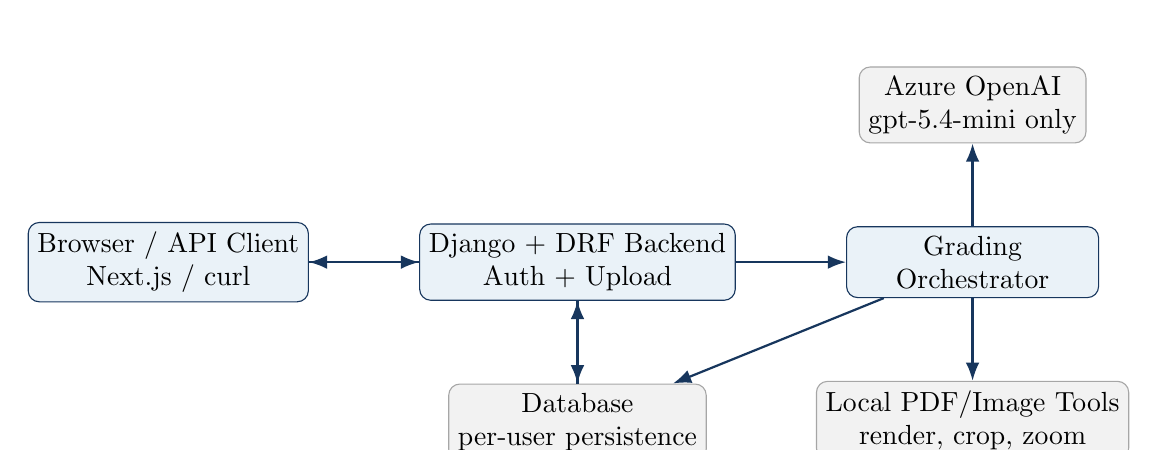
\begin{tikzpicture}[
  node distance=1.05cm and 1.4cm,
  box/.style={rectangle, rounded corners, draw=darkblue, fill=lightblue, align=center, minimum width=3.2cm, minimum height=0.85cm},
  smallbox/.style={rectangle, rounded corners, draw=gray!70, fill=gray!10, align=center, minimum width=2.8cm, minimum height=0.75cm},
  arrow/.style={-Latex, thick, draw=darkblue}
]

\node[box] (client) {Browser / API Client\\Next.js / curl};
\node[box, right=of client] (api) {Django + DRF Backend\\Auth + Upload};
\node[box, right=of api] (orch) {Grading\\Orchestrator};

\node[smallbox, below=of api] (db) {Database\\per-user persistence};
\node[smallbox, below=of orch] (tools) {Local PDF/Image Tools\\render, crop, zoom};
\node[smallbox, above=of orch] (azure) {Azure OpenAI\\gpt-5.4-mini only};

\draw[arrow] (client) -- (api);
\draw[arrow] (api) -- (orch);
\draw[arrow] (api) -- (db);
\draw[arrow] (orch) -- (tools);
\draw[arrow] (orch) -- (azure);
\draw[arrow] (orch) -- (db);
\draw[arrow] (db) -- (api);
\draw[arrow] (api) -- (client);

\end{tikzpicture}
\caption{Split architecture with Next.js frontend, Django/DRF backend, and a framework-agnostic grading engine.}
\end{figure}

\subsection{Main Components}

\begin{itemize}[leftmargin=*]
  \item \textbf{Django REST Framework API}: exposes authentication, grading submission, listing, retrieval, and override endpoints under \code{/api}.
  \item \textbf{Database}: stores users, runs, parsed questions, inferred rubrics, criterion scores, evidence regions, model usage, costs, and teacher overrides.
  \item \textbf{File storage}: stores uploaded PDFs and derived page/crop images in a non-committed volume.
  \item \textbf{PDF/image tool layer}: renders PDF pages, crops regions, zooms/normalizes images, and performs local preprocessing.
  \item \textbf{Azure OpenAI client}: the only external AI model client. It is hard-wired to call the configured \code{gpt-5.4-mini} deployment.
  \item \textbf{Grading orchestrator}: runs the deterministic workflow and bounded agentic inspection loop within a 120-second budget.
\end{itemize}

\section{Why This Is Agentic but Controlled}

The design is agentic because the system does more than call a model once. It decomposes the goal into stages, uses tools, tracks state, validates outputs, and can choose local actions such as crop, zoom, and re-read for difficult handwritten regions. However, it is controlled because the global execution path is fixed and bounded.

\subsection{What Is Fixed}

\begin{itemize}[leftmargin=*]
  \item Request validation and authentication.
  \item PDF preprocessing.
  \item Exam parsing.
  \item Rubric inference.
  \item Student-answer inspection.
  \item Candidate solution interpretation.
  \item Criterion-based grading.
  \item Validation/repair.
  \item Persistence and response formatting.
\end{itemize}

\subsection{What Is Agentic}

The student-answer inspection stage uses bounded ReAct-style behavior. For each question, the inspection agent may select from a small action set: inspect page, locate answer region, crop region, zoom crop, transcribe crop, or mark as missing/unclear. This is where dynamic tool use adds value, because the layout and quality of handwritten answers vary across students.

\begin{notebox}
The system should not log private chain-of-thought reasoning. Logs should record observable actions and decisions, such as \code{rendered page 1}, \code{cropped bbox [120,310,900,620]}, \code{zoomed crop}, or \code{marked question 2 as missing}. This gives traceability without exposing hidden reasoning traces.
\end{notebox}

\section{End-to-end Grading Pipeline}

\begin{figure}[H]
\centering
\resizebox{\textwidth}{!}{%
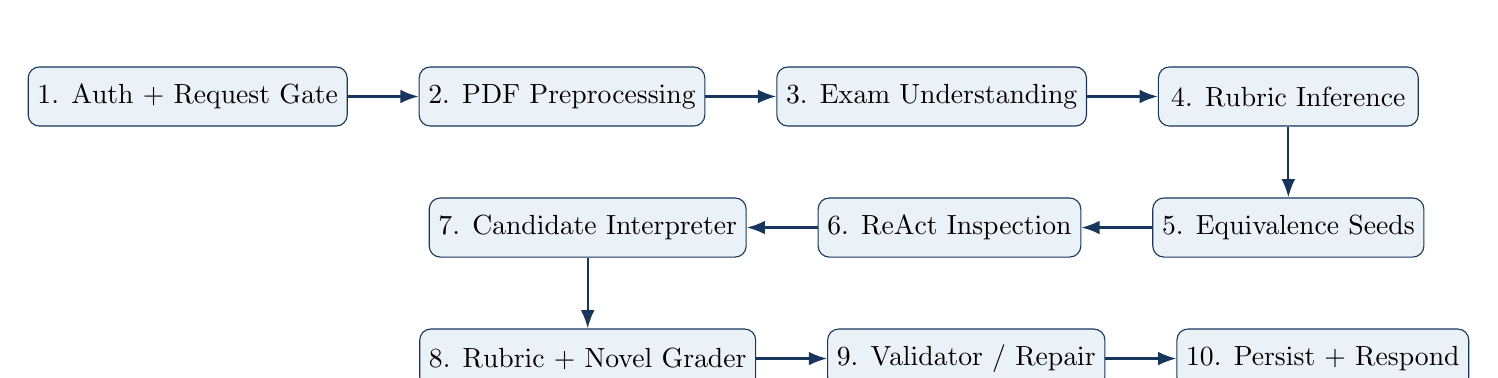
\begin{tikzpicture}[
  node distance=0.9cm,
  stage/.style={rectangle, rounded corners, draw=darkblue, fill=lightblue, align=center, minimum width=3.3cm, minimum height=0.75cm},
  arrow/.style={-Latex, thick, draw=darkblue}
]
\node[stage] (s1) {1. Auth + Request Gate};
\node[stage, right=of s1] (s2) {2. PDF Preprocessing};
\node[stage, right=of s2] (s3) {3. Exam Understanding};
\node[stage, right=of s3] (s4) {4. Rubric Inference};
\node[stage, below=of s4] (s5) {5. Equivalence Seeds};
\node[stage, left=of s5] (s6) {6. ReAct Inspection};
\node[stage, left=of s6] (s7) {7. Candidate Interpreter};
\node[stage, below=of s7] (s8) {8. Rubric + Novel Grader};
\node[stage, right=of s8] (s9) {9. Validator / Repair};
\node[stage, right=of s9] (s10) {10. Persist + Respond};
\draw[arrow] (s1) -- (s2);
\draw[arrow] (s2) -- (s3);
\draw[arrow] (s3) -- (s4);
\draw[arrow] (s4) -- (s5);
\draw[arrow] (s5) -- (s6);
\draw[arrow] (s6) -- (s7);
\draw[arrow] (s7) -- (s8);
\draw[arrow] (s8) -- (s9);
\draw[arrow] (s9) -- (s10);
\end{tikzpicture}%
}
\caption{Final controlled agentic grading pipeline.}
\end{figure}

\subsection{Stage 1: Auth and Request Gate}

\textbf{Input}: authenticated HTTP request containing one exam PDF and one student-answer PDF.

\textbf{Responsibilities}:
\begin{itemize}[leftmargin=*]
  \item Verify bearer token and user identity.
  \item Validate file types, size limits, and PDF readability.
  \item Create a \code{grading_run} row with status \code{running}.
  \item Persist original upload files in a non-committed storage volume.
  \item Start the 120-second hard timeout budget.
\end{itemize}

\textbf{Output}: \code{run_id}, stored file paths, authenticated \code{user_id}, deadline timestamp.

\subsection{Stage 2: PDF Preprocessing}

\textbf{Input}: stored exam PDF and student-answer PDF.

\textbf{Responsibilities}:
\begin{itemize}[leftmargin=*]
  \item Extract text where available.
  \item Render every page to an image at a fixed DPI, e.g., 200-300 DPI.
  \item Generate page thumbnails for cheap layout inspection.
  \item Store page images and metadata.
  \item Optionally deskew, normalize contrast, or resize very large images.
\end{itemize}

\textbf{Output}: normalized document package containing page text, image paths, page count, dimensions, and hashes.

\begin{notebox}
For student answers, page images are the source of truth. Extracted text is advisory only. This is required because several sample student PDFs have zero or unreliable extractable text.
\end{notebox}

\subsection{Stage 3: Exam Understanding Agent}

\textbf{Input}: exam page texts and page images.

\textbf{Responsibilities}:
\begin{itemize}[leftmargin=*]
  \item Identify all questions.
  \item Associate each question with its official solution or mark scheme.
  \item Detect diagrams, equations, and figures that may be needed for grading.
  \item Detect explicit maximum marks if present.
  \item Avoid hard-coding a layout assumption; the exam may be interleaved, sequential, or split into sections.
\end{itemize}

\textbf{Structured output}:
\begin{lstlisting}[language=json]
{
  "questions": [
    {
      "question_id": "1",
      "question_text": "...",
      "official_solution": "...",
      "source_pages": [1],
      "has_diagram_or_formula": true,
      "explicit_max_marks_found": false,
      "explicit_max_marks": null
    }
  ]
}
\end{lstlisting}

\subsection{Stage 4: Rubric Inference Agent}

\textbf{Input}: question text, official solution, optional diagram context, explicit marks if found.

\textbf{Responsibilities}:
\begin{itemize}[leftmargin=*]
  \item Convert each official solution into grading criteria.
  \item Assign marks to criteria.
  \item Preserve source labels: \code{official_explicit}, \code{inferred_from_official_solution}, or \code{system_default}.
  \item Ensure criterion marks sum to the question's maximum marks.
\end{itemize}

\textbf{Policy when marks are absent}: if the exam provides no explicit max marks, use a default configurable value such as 5 marks per question. The output must clearly mark this as \code{max_marks_source = system_default}. This prevents the system from pretending inferred marks are official.

\begin{lstlisting}[language=json]
{
  "question_id": "1",
  "max_marks": 5,
  "max_marks_source": "system_default",
  "rubric_source": "inferred_from_official_solution",
  "criteria": [
    {
      "criterion_id": "1.1",
      "description": "Identifies the slope condition",
      "expected": "b > 1/2",
      "marks": 1.25
    }
  ]
}
\end{lstlisting}

\subsection{Stage 5: Equivalence Seed Generator}

\textbf{Input}: rubric criteria and official solution.

\textbf{Responsibilities}:
\begin{itemize}[leftmargin=*]
  \item Generate obvious equivalent answer forms for fast matching.
  \item Generate canonical expressions where possible.
  \item Define which checks may apply: semantic, symbolic, numeric, unit/dimensional, or conceptual.
\end{itemize}

\textbf{Critical rule}: equivalence seeds are not exhaustive. They are a fast path, not a complete list of all valid student solutions.

\subsection{Stage 6: Student Answer Inspection Agent (Bounded ReAct)}

\textbf{Input}: student page images, question list, rubrics.

\textbf{Responsibilities}:
\begin{itemize}[leftmargin=*]
  \item Inspect student pages and locate where each question is answered.
  \item Use crop/zoom tools when handwriting or formulas are too small or unclear.
  \item Transcribe or summarize the answer region.
  \item Return page and bounding-box evidence for each answer.
  \item Mark unanswered questions as \code{missing} rather than omitting them.
\end{itemize}

\textbf{Allowed tools}:
\begin{itemize}[leftmargin=*]
  \item \code{render_page(pdf_id, page)}
  \item \code{locate_answer_regions(page_image, question_id)}
  \item \code{crop_image(image_id, bbox)}
  \item \code{zoom_image(crop_id, scale)}
  \item \code{transcribe_handwriting(image_id)}
  \item \code{get_question_context(question_id)}
\end{itemize}

\textbf{Bounds}:
\begin{itemize}[leftmargin=*]
  \item Max 4-5 inspection iterations per question.
  \item Max 3 crops per question.
  \item Stop early when sufficient evidence exists.
  \item Respect the shared 120-second deadline.
\end{itemize}

\subsection{Stage 7: Candidate Solution Interpreter}

\textbf{Input}: transcription, evidence regions, question/rubric context.

\textbf{Responsibilities}:
\begin{itemize}[leftmargin=*]
  \item Convert raw transcription into structured student claims.
  \item Extract final answer, intermediate equations, assumptions, and derivation summary.
  \item Preserve uncertain tokens rather than silently normalizing them.
\end{itemize}

\begin{lstlisting}[language=json]
{
  "question_id": "1",
  "student_claims": [
    {"type": "condition", "content": "b > 1/2", "evidence_page": 1},
    {"type": "inequality", "content": "Ia > b + 1", "evidence_page": 1}
  ],
  "final_answer": "b > 1/2 and b + 1 < Ia < 5b - 1",
  "derivation_summary": "Student derives the parameter range using inequalities.",
  "uncertain_parts": []
}
\end{lstlisting}

\subsection{Stage 8: Rubric + Novel Solution Grader}

\textbf{Input}: rubric, equivalence seeds, student claims, transcription, evidence.

\textbf{Responsibilities}:
\begin{itemize}[leftmargin=*]
  \item Award marks criterion by criterion.
  \item Accept exact and equivalent variants quickly.
  \item If the answer does not match known variants, evaluate whether it is a novel but valid solution.
  \item Never require the student to follow the official solution path.
  \item Never award marks without evidence from the student answer.
\end{itemize}

\textbf{Novel solution policy}: known variants are not exhaustive. If a student uses a different derivation that satisfies the criterion mathematically or conceptually, the grader can award full or partial credit and mark \code{match_type = novel_valid_solution}. If verification is inconclusive, the grader sets \code{needs_human_review = true}.

\begin{lstlisting}[language=json]
{
  "criterion_id": "1.3",
  "awarded": 1.25,
  "max": 1.25,
  "match_type": "novel_valid_solution",
  "verification_status": "verified",
  "verification_methods": [
    "rubric_semantic_judge",
    "symbolic_or_numeric_sanity_check",
    "critic_review"
  ],
  "feedback": "The student derived the upper bound using a different but valid inequality transformation.",
  "confidence": 0.82,
  "needs_human_review": false
}
\end{lstlisting}

\subsection{Stage 9: Validator and Repair Agent}

\textbf{Input}: full grading draft.

\textbf{Responsibilities}:
\begin{itemize}[leftmargin=*]
  \item Validate JSON schema.
  \item Ensure every exam question appears exactly once.
  \item Insert missing unanswered questions with 0 marks.
  \item Enforce \code{awarded_marks <= max_marks}.
  \item Recompute totals from per-question scores.
  \item Verify evidence presence for awarded marks.
  \item Flag low-confidence or unclear cases for human review.
  \item Repair minor structural inconsistencies.
\end{itemize}

Structured outputs should be used wherever supported so that model responses conform to a declared JSON Schema. The Azure OpenAI structured-output documentation notes that Azure supports the same subset of JSON Schema as OpenAI for structured outputs. To stay compatible with that subset, schemas should be intentionally simple: use an object as the root, avoid a root-level \code{anyOf}, keep enums explicit, make every required field present, and represent unavailable values with explicit \code{null} fields rather than omitting them. This keeps validation and repair deterministic.

\subsection{Stage 10: Persistence and Response}

\textbf{Input}: validated grading result.

\textbf{Responsibilities}:
\begin{itemize}[leftmargin=*]
  \item Persist final run status, scores, rubrics, evidence, feedback, usage, and cost.
  \item Return the structured grading JSON to the caller.
  \item Make the result retrievable later by the same authenticated user.
\end{itemize}

\section{Output Schema}

The schema is designed for completeness, traceability, and defensibility. It makes the source of marks explicit and records whether an answer was matched exactly, matched through known variants, or accepted as a novel valid solution.

\begin{lstlisting}[language=json]
{
  "grading_id": "uuid",
  "status": "completed",
  "model_deployment": "gpt-5.4-mini",
  "total_score": 7.25,
  "max_score": 10.0,
  "duration_ms": 87342,
  "questions": [
    {
      "question_id": "1",
      "awarded_marks": 4.25,
      "max_marks": 5.0,
      "rubric_source": "inferred_from_official_solution",
      "max_marks_source": "system_default",
      "feedback": "Good derivation overall. Final notation should be clearer.",
      "confidence": 0.84,
      "needs_human_review": false,
      "criterion_scores": [
        {
          "criterion_id": "1.1",
          "awarded": 1.25,
          "max": 1.25,
          "match_type": "equivalent_variant",
          "verification_status": "verified",
          "feedback": "The slope condition was correctly identified.",
          "evidence": {
            "page": 1,
            "bbox": [120, 310, 900, 620]
          }
        }
      ]
    }
  ]
}
\end{lstlisting}

\section{API Design}

\subsection{Authentication Endpoints}

\begin{longtable}{p{0.24\textwidth}p{0.18\textwidth}p{0.48\textwidth}}
\toprule
\textbf{Endpoint} & \textbf{Auth} & \textbf{Purpose} \\
\midrule
\code{POST /auth/register} & No & Create user with email and password. Store only password hash. \\
\code{POST /auth/login} & No & Validate credentials and return bearer token. \\
\code{GET /auth/me} & Yes & Optional sanity endpoint for current user. \\
\bottomrule
\end{longtable}

\subsection{Health Endpoint}

\begin{longtable}{p{0.24\textwidth}p{0.18\textwidth}p{0.48\textwidth}}
\toprule
\textbf{Endpoint} & \textbf{Auth} & \textbf{Purpose} \\
\midrule
\code{GET /health} & No & Lightweight liveness check for Docker and local smoke tests. It should confirm that the API process is running without requiring Azure credentials or making an LLM call. \\
\bottomrule
\end{longtable}

\subsection{Grading Endpoints}

\begin{longtable}{p{0.26\textwidth}p{0.14\textwidth}p{0.50\textwidth}}
\toprule
\textbf{Endpoint} & \textbf{Auth} & \textbf{Purpose} \\
\midrule
\code{POST /gradings} & Yes & Upload exam PDF and student-answer PDF; run grading synchronously within the 120-second budget. \\
\code{GET /gradings} & Yes & List past grading runs owned by the authenticated user. \\
\code{GET /gradings/\{id\}} & Yes & Retrieve a single grading run owned by the authenticated user. \\
\code{PATCH /gradings/\{id\}/override} & Yes & Optional bonus: teacher/user can override a question mark with a reason. \\
\bottomrule
\end{longtable}

\subsection{Example Curl Flow}

\begin{lstlisting}[language=bash]
# Register
curl -X POST http://localhost:8000/auth/register \
  -H "Content-Type: application/json" \
  -d '{"email":"teacher@example.com","password":"strong-password"}'

# Login
TOKEN=$(curl -s -X POST http://localhost:8000/auth/login \
  -H "Content-Type: application/json" \
  -d '{"email":"teacher@example.com","password":"strong-password"}' \
  | jq -r .access_token)

# Submit grading
curl -X POST http://localhost:8000/gradings \
  -H "Authorization: Bearer $TOKEN" \
  -F "exam_pdf=@samples/Q&A/Homework_3_sols.pdf" \
  -F "student_pdf=@samples/studentAnswers/3u2021152663.pdf"
\end{lstlisting}

\section{Database Design}

A relational database is recommended because ownership, grading runs, questions, criteria, scores, evidence, and overrides have clear relationships. SQLite with a Docker volume is acceptable for this take-home; Postgres is also fine. The important requirement is that data persists across container restarts and is scoped per user.

\begin{longtable}{p{0.25\textwidth}p{0.65\textwidth}}
\toprule
\textbf{Table} & \textbf{Fields / Purpose} \\
\midrule
\code{users} & \code{id}, \code{email}, \code{password_hash}, timestamps. \\
\code{grading_runs} & \code{id}, \code{user_id}, status, file paths, total score, max score, deployment, duration, token usage, cost, timestamps. \\
\code{questions} & Parsed question text, official solution, source pages, max marks, source labels. \\
\code{rubric_criteria} & Criterion id, description, expected answer, marks, source. \\
\code{student_answers} & Transcription, final answer, derivation summary, missing/answered status, uncertainty flags. \\
\code{question_grades} & Awarded marks, max marks, feedback, confidence, human-review flag. \\
\code{criterion_grades} & Criterion-level scores, match type, verification status, feedback. \\
\code{evidence_regions} & Page number, bbox, crop path, zoom flag, linked criterion/question. \\
\code{teacher_overrides} & Old score, new score, reason, user id, timestamp. \\
\code{model_calls} & Per-call deployment, prompt/completion tokens, duration, status, cost. \\
\bottomrule
\end{longtable}

\section{Recommended Code Structure}

\begin{lstlisting}
project/
|-- backend/
|   |-- Dockerfile
|   |-- requirements.txt
|   |-- app/
|   |   |-- main.py
|   |   |-- api/
|   |   |   |-- auth.py
|   |   |   `-- gradings.py
|   |   |-- core/
|   |   |   |-- config.py
|   |   |   |-- security.py
|   |   |   |-- logging.py
|   |   |   `-- timeouts.py
|   |   |-- db/
|   |   |   |-- models.py
|   |   |   |-- session.py
|   |   |   `-- repositories.py
|   |   |-- services/
|   |   |   |-- azure_client.py
|   |   |   |-- cost_logger.py
|   |   |   |-- file_storage.py
|   |   |   |-- pdf_preprocessor.py
|   |   |   `-- grading_orchestrator.py
|   |   |-- agents/
|   |   |   |-- exam_understanding.py
|   |   |   |-- rubric_inference.py
|   |   |   |-- equivalence.py
|   |   |   |-- student_inspection.py
|   |   |   |-- candidate_interpreter.py
|   |   |   |-- grader.py
|   |   |   `-- validator.py
|   |   |-- tools/
|   |   |   |-- render_pdf.py
|   |   |   |-- crop_image.py
|   |   |   |-- zoom_image.py
|   |   |   `-- math_checks.py
|   |   `-- schemas/
|   |       |-- auth.py
|   |       |-- rubric.py
|   |       |-- grading.py
|   |       `-- api.py
|   `-- tests/
|       |-- unit/
|       |-- integration/
|       `-- fixtures/
|-- docker-compose.yml
|-- .env.example
|-- .gitignore
`-- README.md
\end{lstlisting}

\subsection{Library Choices}

\begin{longtable}{p{0.25\textwidth}p{0.65\textwidth}}
\toprule
\textbf{Library} & \textbf{Purpose} \\
\midrule
\code{django}, \code{djangorestframework} & Backend HTTP API, routing, request parsing, permissions, and serialization. \\
\code{pydantic} & Internal structured grading schemas used by the grading engine and Azure structured outputs. \\
\code{django ORM} & Database models and persistence. \\
\code{Django migrations} & Schema evolution. \\
\code{Django password hashing} & Secure password storage for the custom user model. \\
\code{PyJWT} & JWT creation and verification. \\
\code{Django multipart parsers} & File upload support in the grading API. \\
\code{pypdfium2} or \code{PyMuPDF} & PDF page rendering and text extraction. \\
\code{Pillow} & Image manipulation, cropping, resizing, and saving. \\
\code{opencv-python-headless} & Optional deskew/contrast normalization. \\
\code{openai} & Azure OpenAI client configured with endpoint, key, API version, and deployment. \\
\code{pytest}, \code{httpx} & Unit and integration tests. \\
\code{ruff}, \code{mypy} & Optional linting and static checks. \\
\bottomrule
\end{longtable}

\begin{riskbox}
Do not add a second cloud OCR provider or alternate LLM service unless explicitly permitted. It risks violating the model/deployment restriction. Use local rendering/cropping tools and the single provisioned Azure OpenAI deployment.
\end{riskbox}

\section{Azure OpenAI Client Rules}

The Azure client must be a narrow wrapper around the provisioned deployment. Azure OpenAI API calls refer to a \emph{deployment name}, not a general model selector. The assignment quickstart specifies the exact deployment value \code{gpt-5.4-mini}; therefore the implementation should read \code{AZURE_OPENAI_DEPLOYMENT} from the environment, validate it against the assignment value, and use that value for every call. The code must not expose a per-request model parameter, must not call embeddings/OCR/other model deployments, and must not implement fallback behavior.

\begin{notebox}
If the assignment provider changes the deployment name in a future quickstart, update \code{.env.example} and the validation constant together. Do not silently route to another deployment. The current bundle says the exact value is \code{gpt-5.4-mini}.
\end{notebox}

\begin{lstlisting}[language=Python]
ALLOWED_DEPLOYMENT = "gpt-5.4-mini"  # from API_QUICKSTART.pdf

class AzureGraderClient:
    def __init__(self, settings: Settings):
        self.client = AzureOpenAI(
            api_key=settings.azure_openai_api_key,
            azure_endpoint=settings.azure_openai_endpoint,
            api_version=settings.azure_openai_api_version,
        )
        self.deployment = settings.azure_openai_deployment
        if self.deployment != ALLOWED_DEPLOYMENT:
            raise RuntimeError(
                "Invalid deployment. Use AZURE_OPENAI_DEPLOYMENT "
                "from API_QUICKSTART.pdf only."
            )

    async def complete_json(self, *, messages, schema, timeout_budget):
        # Always use self.deployment as the Azure deployment name.
        # Do not accept model/deployment overrides from callers.
        ...
\end{lstlisting}

\section{Timeout and Cancellation Strategy}

The grading endpoint must return within 120 seconds or respond with HTTP 504. This must be real cancellation, not merely a request parameter.

\subsection{Budget Allocation}

\begin{longtable}{p{0.36\textwidth}p{0.18\textwidth}p{0.36\textwidth}}
\toprule
\textbf{Stage} & \textbf{Suggested Budget} & \textbf{Notes} \\
\midrule
Request validation and file save & 5 s & Fast local work. \\
PDF preprocessing & 10-20 s & Depends on page count and DPI. \\
Exam parsing + rubric inference & 20-30 s & One model call where possible. \\
Student inspection & 25-45 s & One model call plus crop/zoom only if needed. \\
Grading + validation & 25-35 s & One model call plus schema validation. \\
Safety margin & 5-10 s & Needed for cleanup and DB commit. \\
\bottomrule
\end{longtable}

\subsection{Cancellation Implementation}

Use \code{asyncio.timeout}, \code{anyio.fail_after}, or an equivalent cancellation boundary around the full orchestrator. Local subprocesses for rendering must be killed if the deadline expires. LLM calls must use client-side timeout and be wrapped by the same global deadline.

\begin{lstlisting}[language=Python]
async def submit_grading(...):
    try:
        async with asyncio.timeout(120):
            result = await orchestrator.grade(...)
            return result
    except TimeoutError:
        await repo.mark_run_failed(run_id, reason="timeout")
        raise HTTPException(status_code=504, detail="Grading timed out")
\end{lstlisting}

\section{Structured Logging and Cost Tracking}

The backend should log one structured JSON line per important event. This makes the container inspectable with \code{docker compose logs -f}. Logs must never include passwords, secrets, full bearer tokens, or raw API keys.

\subsection{Required Log Events}

\begin{itemize}[leftmargin=*]
  \item \code{grading.submitted}
  \item \code{pdf.preprocessed}
  \item \code{llm.call.started}
  \item \code{llm.call.completed}
  \item \code{llm.call.failed}
  \item \code{grading.completed}
  \item \code{grading.timeout}
  \item \code{grading.override.created}
\end{itemize}

\subsection{Example Log Line}

\begin{lstlisting}[language=json]
{
  "event": "llm.call.completed",
  "run_id": "8cf4...",
  "user_id": "3a12...",
  "stage": "student_inspection",
  "deployment": "gpt-5.4-mini",
  "input_tokens": 18234,
  "output_tokens": 1450,
  "duration_ms": 9210,
  "cost_usd": 0.0127,
  "status": "ok"
}
\end{lstlisting}

\subsection{Cost Formula}

The assignment asks for per-run cost calculation from the published Azure OpenAI per-token rates for the deployed model. Because published prices may change, the implementation should keep rates in configuration and document where to update them.

\begin{lstlisting}[language=Python]
def compute_cost_usd(input_tokens, output_tokens, settings):
    return (
        input_tokens / 1_000_000 * settings.azure_input_usd_per_1m_tokens
        + output_tokens / 1_000_000 * settings.azure_output_usd_per_1m_tokens
    )
\end{lstlisting}

Recommended environment variables:

\begin{lstlisting}
AZURE_OPENAI_INPUT_USD_PER_1M_TOKENS=...
AZURE_OPENAI_OUTPUT_USD_PER_1M_TOKENS=...
\end{lstlisting}

The README should instruct the developer to set these values from the current Azure OpenAI pricing page for the provided deployment. The official Azure OpenAI pricing page is token-based and may change over time, so keeping this configurable avoids hard-coding stale prices.

For the bonus cost log to be trustworthy, the backend should choose one explicit behavior:
\begin{itemize}[leftmargin=*]
  \item \textbf{Strict mode}: fail startup if pricing environment variables are missing.
  \item \textbf{Permissive mode}: run grading but log \code{cost_usd = null} and emit a clear warning that pricing variables were not configured.
\end{itemize}
Strict mode is preferred for final submission because the assignment specifically asks for exact per-run cost calculation when this bonus is implemented.

\section{Prompting and Agent Instructions}

Prompts should be short, task-specific, and schema-bound. Each agent should have a narrow role. Avoid asking one model call to parse the exam, infer a rubric, inspect handwriting, grade, validate, and repair all at once.

\subsection{Exam Understanding Prompt Skeleton}

\begin{lstlisting}
You are an exam-structure parser.
Given the exam PDF pages as text and/or images, extract all questions and the official solution or mark-scheme content associated with each question.
Do not grade the student. Do not infer marks except detecting explicit marks.
Return only JSON matching the provided schema.
\end{lstlisting}

\subsection{Rubric Inference Prompt Skeleton}

\begin{lstlisting}
You are a rubric builder.
For each question and official solution, construct grading criteria.
If marks are explicit, preserve them and set rubric_source="official_explicit".
If marks are not explicit, infer criteria from the solution and set rubric_source="inferred_from_official_solution".
If max marks are absent, use the configured default and set max_marks_source="system_default".
Return only JSON matching the rubric schema.
\end{lstlisting}

\subsection{Student Inspection Prompt Skeleton}

\begin{lstlisting}
You are a student-answer inspection agent.
Your goal is to locate, crop if needed, and transcribe the student's answer for each question.
Use the available local tools when handwriting is too small, skewed, or unclear.
Do not grade. Do not infer marks.
Always return page numbers and bounding boxes for evidence.
If an answer is absent, return status="missing".
If handwriting remains unclear, record uncertain_tokens and set needs_human_review=true.
\end{lstlisting}

\subsection{Grading Prompt Skeleton}

\begin{lstlisting}
You are a criterion-based grading agent.
Grade the student answer against the rubric criteria.
The accepted variant list is not exhaustive.
Do not require the same solution path as the official solution.
Award marks if the student's reasoning satisfies the criterion mathematically or conceptually.
Do not award marks without evidence from the student answer.
If a novel solution may be correct but cannot be verified confidently, set needs_human_review=true.
Return only JSON matching the grading schema.
\end{lstlisting}

\section{Testing Strategy}

Testing is divided into unit tests, integration tests, sample-based smoke tests, and rejection-rule checks.

\subsection{Unit Tests}

\begin{longtable}{p{0.32\textwidth}p{0.58\textwidth}}
\toprule
\textbf{Area} & \textbf{Tests} \\
\midrule
Password hashing & Raw passwords are never stored; correct password verifies; wrong password fails. \\
JWT auth & Token creation, token expiration, invalid token rejection. \\
User scoping & User A cannot list or retrieve User B's grading runs. \\
PDF preprocessing & Page count extraction, image rendering, invalid PDF rejection, file cleanup on failure. \\
Schema validation & Missing required fields fail; valid agent outputs pass; totals are recomputed. \\
Rubric normalization & Criterion marks sum to max marks; default marks are labeled as default. \\
Novel solution flags & Non-variant answers can be marked as \code{novel_valid_solution}; inconclusive cases trigger human review. \\
Cost calculation & Given token counts and rates, computed cost matches expected formula. \\
Timeout utility & Artificial long-running coroutine is cancelled and maps to 504. \\
\bottomrule
\end{longtable}

\subsection{Integration Tests}

\begin{itemize}[leftmargin=*]
  \item Start the service with Docker Compose.
  \item Register a user.
  \item Log in and obtain a token.
  \item Submit a sample exam and one student PDF.
  \item Assert HTTP 200 or 504 only under simulated timeout.
  \item Assert every question appears in the result.
  \item Assert total score equals the sum of question scores.
  \item Assert result is persisted and retrievable.
  \item Assert unauthenticated grading submission returns 401.
  \item Assert another user cannot retrieve the first user's grading result.
\end{itemize}

\subsection{Sample-based Smoke Tests}

The sample bundle should be used to verify robustness rather than absolute grading accuracy. For each of the seven student PDFs:

\begin{itemize}[leftmargin=*]
  \item The backend should complete or return a real 504 under controlled timeout.
  \item The result should include all exam questions.
  \item Blank or missing answers should appear with 0 marks, not disappear.
  \item Each awarded mark should have page-level or region-level evidence where possible.
  \item No score should exceed its maximum.
\end{itemize}

\subsection{Rejection-rule Test Checklist}

\begin{lstlisting}[language=bash]
# Clean clone smoke
cp .env.example .env
# fill required env vars manually or in CI secret store
docker compose up --build

# Health check
curl http://localhost:8000/health

# Register/login/grade/list/retrieve flow
pytest backend/tests/integration/test_required_flow.py

# Ensure no secrets committed
git ls-files | grep -E '(^|/)(.env|*.sqlite|*.db|uploads/)'
\end{lstlisting}

\section{README Requirements}

The root README should include the following sections:

\begin{enumerate}[leftmargin=*]
  \item Project overview.
  \item Architecture diagram or short architecture description.
  \item How to run with \code{docker compose up}.
  \item Required environment variables, copied from \code{API_QUICKSTART.pdf}: \code{AZURE_OPENAI_API_KEY}, \code{AZURE_OPENAI_ENDPOINT}, \code{AZURE_OPENAI_DEPLOYMENT}, and \code{AZURE_OPENAI_API_VERSION}.
  \item A short note telling maintainers to read \code{API_QUICKSTART.pdf} before changing Azure client code.
  \item API endpoint documentation with curl examples.
  \item Database and persistence explanation.
  \item Grading pipeline explanation.
  \item Model restriction: only \code{gpt-5.4-mini} deployment is called.
  \item Timeout behavior: 120-second hard limit and HTTP 504.
  \item Logging and cost calculation.
  \item Testing instructions.
  \item Known limitations.
  \item How AI tools were used during development.
\end{enumerate}

\section{Known Limitations}

\begin{itemize}[leftmargin=*]
  \item If the official mark allocation is not explicit, the rubric is inferred. The output labels this clearly.
  \item Handwriting recognition may be uncertain for low-quality scans. Such cases are flagged for human review.
  \item The system grades for structure, consistency, completeness, and evidence-based reasoning; it does not guarantee perfect marking accuracy.
  \item Symbolic equivalence checks are best effort. Some mathematically valid transformations may require semantic judging or human review.
  \item The frontend remains intentionally thin and relies on the backend for the real grading workflow, validation, and persistence rules.
  \item Multi-student support is not in the first required scope, but the schema can support it later.
\end{itemize}

\section{Implementation Plan}

\subsection{Phase 1: Rejection-safe Backend}

\begin{itemize}[leftmargin=*]
  \item Create Django project and REST API app structure.
  \item Implement register/login/JWT.
  \item Implement persistent database and user scoping.
  \item Add required grading endpoints with placeholder result.
  \item Add Docker Compose and README skeleton.
\end{itemize}

\subsection{Phase 2: PDF and Azure Integration}

\begin{itemize}[leftmargin=*]
  \item Implement file upload storage.
  \item Implement PDF text extraction and page rendering.
  \item Read \code{API_QUICKSTART.pdf}, then implement the Azure client wrapper locked to \code{AZURE_OPENAI_DEPLOYMENT = gpt-5.4-mini} with no per-call override or fallback.
  \item Add structured-output schemas.
\end{itemize}

\subsection{Phase 3: Grading Pipeline}

\begin{itemize}[leftmargin=*]
  \item Exam understanding agent.
  \item Rubric inference agent.
  \item Student inspection agent with bounded crop/zoom actions.
  \item Candidate interpreter.
  \item Criterion-based grader and validator.
\end{itemize}

\subsection{Phase 4: Reliability and Polish}

\begin{itemize}[leftmargin=*]
  \item Add timeout cancellation and 504 path.
  \item Add structured logging and cost calculation.
  \item Add tests.
  \item Add optional teacher override.
  \item Finalize README.
\end{itemize}

\section{Follow-up Call Defense Points}

If asked to defend the design:

\begin{itemize}[leftmargin=*]
  \item \textbf{Why agentic?} Because grading requires document understanding, handwritten answer localization, rubric inference, novel solution validation, and structured validation. A single prompt is less reliable.
  \item \textbf{Why not fully autonomous?} Because reliability and rejection constraints matter. The workflow is fixed, and the agentic part is bounded to inspection/crop/zoom decisions.
  \item \textbf{How are absent marks handled?} Default marks are used only when official marks are absent, and the source is labeled as \code{system_default}.
  \item \textbf{How are different correct solutions handled?} Known variants are not exhaustive. The grader evaluates whether student claims satisfy the rubric even if the derivation differs.
  \item \textbf{How is handwriting handled?} Student PDFs are rendered to images; the inspection agent can crop and zoom answer regions and returns page/bbox evidence.
  \item \textbf{How is the 120-second rule enforced?} The entire orchestrator runs under a global cancellation boundary, and timeout returns HTTP 504.
  \item \textbf{How is model usage controlled?} The Azure client has one deployment value and no fallback path.
\end{itemize}

\section{References and Documentation Sources}

\begin{itemize}[leftmargin=*]
  \item Zanista take-home assignment PDF, \emph{Engineering Intern - Take-Home: Build a minimal AI exam grader}.
  \item Zanista \code{API_QUICKSTART.pdf}: Azure OpenAI endpoint, API version, environment variables, and exact \code{gpt-5.4-mini} deployment rule.
  \item OpenAI API documentation, \emph{Structured Outputs}: \url{https://developers.openai.com/api/docs/guides/structured-outputs}
  \item Microsoft Learn, \emph{Use vision-enabled chat models with Azure OpenAI}: \url{https://learn.microsoft.com/en-us/azure/foundry/openai/how-to/gpt-with-vision}
  \item Microsoft Learn, \emph{Azure OpenAI structured outputs}: \url{https://learn.microsoft.com/en-us/azure/foundry/openai/how-to/structured-outputs}
  \item Django documentation, \emph{Customizing authentication}: \url{https://docs.djangoproject.com/en/stable/topics/auth/customizing/}
  \item Docker documentation, \emph{docker compose up}: \url{https://docs.docker.com/reference/cli/docker/compose/up/}
  \item Azure pricing page for current Azure OpenAI per-token rates: \url{https://azure.microsoft.com/en-us/pricing/details/azure-openai/}
\end{itemize}

\end{document}
